\documentclass{erauthesis}
\department{Mechanical Engineering}
\chair{Eric Coyle, Ph.D}
\dean{James Gregory, Ph.D.}
\dgc{Lon Moeller, J.D.}
\depchair{Patrick Currier, Ph.D.}
\advisortitle{Committee chair}
\usepackage{graphicx}
\usepackage{amsmath}
\usepackage{amssymb}
\usepackage{textcomp, gensymb}
\usepackage{array}
\usepackage{enumitem}
\usepackage{xcolor}
\usepackage{algorithm}
\usepackage{algpseudocode}

\usepackage{subcaption} % for multiple image figures
% \usepackage[style=authoryear]{biblatex} % or numeric, apa, etc.
% \addbibresource{Dissertation.bib}         % your Zotero export

% pkgs for .mermaid chart
\usepackage{tikz}
\usetikzlibrary{shapes.geometric, arrows}

% acronyms
\usepackage[nolist]{acronym} 

% preamble for Lit-review tables:
\usepackage{tabularx,ragged2e,makecell}
\renewcommand\theadfont{\bfseries}
\renewcommand\cellalign{tl} % top-left for makecell
\newcolumntype{L}[1]{>{\RaggedRight\arraybackslash}p{#1}}
\newcolumntype{Y}{>{\RaggedRight\arraybackslash}X}

\title{A STUDY IN OBJECT DETECTION AND CLASSIFICATION
PERFORMANCE BY SENSING MODALITY FOR AUTONOMOUS
SURFACE VESSELS} % the title should be included here
\author{Daniel P. Lane} 
\graduation{December}{2025}
\advisor {Eric Coyle} %Committe chair


\coadvisor{Subhradeep Roy} % If you do not have a co-advisor, delete this whole command

\committememzero{Xxxx X. Xxxxxxxxx, Ph.D.} % If you have a co-advisor, do not edit this member name
%% Enter the name of the committee members
\committememone{Patrick Currier}
\committememtwo{Monica Garcia}
\committememthree{Jianhua Liu}
\committememfour{TBD}



%\signaturepush{-2.0}									

\usepackage{subfiles} % Best loaded last in the preamble

\begin{document}


\frontmatter

\maketitle

% \makesignature
\makeatletter 
\advance\fau@frontstage by 1  % Skip signature page but maintain counter
% \makeanother
\begin{acronym}[GB-CACHE] % Give the longest label here so that the list is nicely aligned
\acro{AGS}{autonomous ground system}
\acro{ASV}{autonomous surface vessel}
\acro{USV}{unmanned surface vessel}
\acro{ERAU}{Embry-Riddle Aeronautical University}
\acro{GB-CACHE}{grid-based clustering and concave hull extraction}
\acro{GPS}{Global Positioning System}
\acro{WAM-V}{wave-adaptive modular vessel}
\acro{SDR}{standard dynamic range}
\acro{HDR}{high dynamic range}
\acro{DOL-HDR}{digital-overlap HDR}
\acro{IMU}{inertial measurement unit}
\acro{INS}{inertial navigation system}
\acro{IoU}{intersection over union}
\acro{LiDAR}{light detection and ranging}
\acro{pps}{points per second}
\acro{mAP}{mean average precision}
\acro{MPC}{model predictive control}
\acro{RGB}{red, green, blue}
\acro{ROI}{region of interest}
\acro{ROS}{Robot Operating System}
\acro{YOLO}{You Only Look Once}
\acro{YOLOv8}{You Only Look Once ver. 8.0}
\acro{LWIR}{long-wave infrared}
\acro{FPS}{frames per second}
\acro{EFL}{effective focal length}
\acro{FOV}{field of view}
\acro{LAN}{local area network}
\acro{SEI}{supplemental enhancement information}
\acro{NAL}{network abstraction layer}
\acro{NTP}{Network Time Protocol}
\acro{PTP}{Precision Time Protocol}
\acro{RTP}{Real-time Transport Protocol}
\acro{RTSP}{Real-time Streaming Protocol}
\acro{UDP}{User Datagram Protocol}

\end{acronym}

\begin{acknowledgements}
% \raggedright
I would like to express my deepest gratitude to my friends, family, and especially my parents, whose unwavering love, encouragement, and support have sustained me throughout my academic journey. Their belief in me has been a constant source of strength and motivation.

I am sincerely thankful to my advisor, Dr. Coyle, for his mentorship and steady guidance throughout this research. He has taught me lessons both in and beyond the classroom that will stay with me for a lifetime, and for that, I will be forever grateful.

I would also like to extend a special thanks to my co-advisor, Dr. Roy, who first introduced me to the world of academic research rigor. His guidance shaped the foundation of my development as a researcher and helped me grow into the kind of professional and scholar I aspired to become.

Finally, I wish to acknowledge the faculty and staff of the Department of Mechanical Engineering for their continued support of my academic and professional growth. 
Their commitment to excellence in teaching and research has profoundly influenced my development as both a student and an educator.

\vspace{3mm}

This work was supported in part by NEEC grant N00174-22-1-0012 through NUWC Keyport.
Any opinions, findings, conclusions, or recommendations expressed in this material are those of the authors and do not necessarily reflect the views of the Department of the Navy or Office of Naval Research.
\end{acknowledgements}

\begin{abstract}
	% \raggedright Researcher: Daniel P. Lane
 % \\Title: A study in object detection and classification performance by sensing modality for autonomous surface vessels \\Institution:	Embry-Riddle Aeronautical University\\Degree:	Doctor of Philosophy in Mechanical Engineering\\Year:	2025 \\
 This research addresses the critical gap in quantitative performance comparison between \ac{LiDAR} and vision-based sensing for real-time maritime object detection on autonomous surface vessels.
 Using \ac{ERAU}'s Minion platform and 2024 Maritime RobotX Challenge data, this study evaluates \ac{GB-CACHE} \ac{LiDAR} processing against \ac{YOLO} vision detection across six maritime object categories. The methodology encompasses real-time performance analysis, multi-sensor calibration, and sensor fusion for bounding box confidence integration.
 Performance metrics include precision, recall, \ac{mAP}, training requirements, and computational efficiency. 
 % Results demonstrate [key performance finding] and establish [fusion outcome]. 
 The research provides quantitative baselines for maritime sensing modality selection and validated calibration procedures enabling improved autonomous navigation in complex maritime environments.
 
 % Lorem ipsum dolor sit amet... This is a summative abstract, not just a list of topics.  Include relevant information including conclusions and recommendations.  Limit to 150 words; spell out abbreviations; citations not needed.

\end{abstract}
\pagetableofcontents
\clearpage
\listoftables					% Or \nolistoftables if there are no 
\clearpage
\listoffigures					% Or \nolistoffigures if there are no 




\mainmatter
\newpage
\chapter{Introduction}
\subfile{sections/introduction}

\section{Significance of Study} \label{significance_of_study}
\subfile{sections/significance_of_study}

\section{Problem Statement: Performance Comparison Gap} \label{problem_statement1}
\subfile{sections/problem_statement1}

%%%%%%%%%%%%%%%%%%%%%%%%%%%%%%%%%%%%%%%%%%%%%%%%%%%
%%%%%%%%%%%%%%%%%%%%%%%%%%%%%%%%%%%%%%%%%%%%%%%%%%%
%%%%%%%%%%%%%%%%%%%%%%%%%%%%%%%%%%%%%%%%%%%%%%%%%%%
\chapter{Literature Review} \label{litReview}
% \subfile{sections/literatureReview_new}
\subfile{sections/literatureReview_old}

%%%%%%%%%%%%%%%%%%%%%%%%%%%%%%%%%%%%%%%%%%%%%%%%%%%
%%%%%%%%%%%%%%%%%%%%%%%%%%%%%%%%%%%%%%%%%%%%%%%%%%%
%%%%%%%%%%%%%%%%%%%%%%%%%%%%%%%%%%%%%%%%%%%%%%%%%%%
\chapter{Sensing Platform} \label{sensing_platform}
\subfile{sections/sensing_platform_intro}

\section{Perception Geometry} \label{perception_geometry}
\subfile{sections/perception_geometry}

\section{Sensors} \label{sensors}
% \subfile{sections/sensors}

\subsection{LiDAR} \label{sensors_LiDAR}
\subfile{sections/LiDAR}

\subsection{Visible Spectrum Cameras} \label{visual_cameras}
\subfile{sections/cameras}

\subsection{PinPoint GPS/INS} \label{sensors_GPS}
\subfile{sections/pinpoint}

\section{Compute Hardware and Network} \label{sec:Atlas_LAN}
\subfile{sections/hardware}

\section{Sensor Calibration} \label{sec:calibration}
\subfile{sections/calibration}

\begin{figure}[htbp]
    \centering
    \includegraphics[width=0.7\linewidth]{Images/tf_tree_1.png}
    \caption{Transform hierarchy for Minion: the GPS-defined \texttt{map} frame anchors the ROS TF tree used for LiDAR–camera projection and sensor fusion.}
    \label{fig:tf_tree}
\end{figure}

%%%%%%%%%%%%%%%%%%%%%%%%%%%%%%%%%%%%%%%%%%%%%%%%%%%%%%%%%%%%%%%%%%%%
\subsection{Spatial Calibration} \label{spatial_calibration}

Before data from the camera and \ac{LiDAR} sensors can be combined, each device must be spatially calibrated through intrinsic and extrinsic transformations.  
This process establishes the geometric relationships required to express all sensor measurements in a unified coordinate frame, enabling accurate projection of \ac{LiDAR} points onto the camera image plane.

Calibration begins with determining the camera’s intrinsic parameters, followed by estimation of the extrinsic transformation that defines the rigid-body relationship between the camera and each \ac{LiDAR} sensor.  
The following sections describe the methods and results of this calibration process.

%%%%%%%%%%%%%%%%%%%%%%%%%%%%
\subsubsection{Extrinsic Calibration} \label{extrinsic_tform}
\subfile{sections/extrinsic_tform}

\begin{figure}[htbp]
    \centering
    \includegraphics[width=0.9\linewidth]{Images/Lidar2Lidar.png}
    \caption{Example of LiDAR–LiDAR alignment.}
    \label{fig:Lidar2Lidar}
\end{figure}

%%%%%%%%%%%%%%%%%%%%%%%%%%%%
\subsubsection{Camera Intrinsics} \label{camera_intrinsics}
\subfile{sections/cam_intrinsics}

\begin{figure}[htbp]
\centering
\makebox[\textwidth][c]{%
    \begin{subfigure}[t]{0.3\textwidth}
        \centering
        \includegraphics[width=\textwidth]{Images/cam_calib_1.png}
        \caption{A single example of detected and reprojected checkerboard corners.}
        \label{fig:cam_calib_1}
    \end{subfigure}
    \hspace{2em}
    \begin{subfigure}[t]{0.625\textwidth}
        \centering
        \includegraphics[width=\textwidth]{Images/cam_calib_2.png}
        \caption{Reprojection of sample target poses into the 3D world frame after calibration.}
        \label{fig:cam_calib_2}
    \end{subfigure}%
}
\caption{Checkerboard images are processed to detect corners. Agreement between detected (green circles) and reprojected (red crosses) points demonstrates corner localization and mapping of the image coordinate system.(left), which enable intrinsic parameters to be estimated and validated by reprojecting known targets into 3D space (right).}
\label{fig:cam_calib}
\end{figure}


\subsubsection{Camera to LiDAR Extrinsic Calibration} \label{camLidar_calib}
\subfile{sections/camlidar_calib}

\begin{figure}[htbp]
\centering
\makebox[\textwidth][c]{
    \begin{subfigure}[t]{0.44\textwidth}
        \centering
        \includegraphics[width=\textwidth]{Images/checkerboard.png}
        \caption{Composite image of multiple checkerboard target locations.}
        \label{fig:checkerboard}
    \end{subfigure}
    \hspace{2em}
    \begin{subfigure}[t]{0.44\textwidth}
        \centering
        \includegraphics[width=\textwidth]{Images/LiDAR_calib.png}
        \caption{Composite of checkerboard locations in the LiDAR reference frame.}
        \label{fig:LiDAR_calib}
    \end{subfigure}
}
\caption{Checkerboard targets used for camera intrinsic (left) and LiDAR extrinsic (right) calibration. Red dots mark detected corner points transformed into the LiDAR frame using the initial extrinsic estimate.}
\label{fig:camLidar_calib}
\end{figure}

%%%%%%%%%%%%%%%%%%%%%%%%%%%%%%%%%%%%%%%%%%%%%%%%%%%
\subsection{Results: Spatial Calibration} \label{sec:spatial_calib_results}
\subsubsection{LiDAR–LiDAR Calibration} \label{results_lidarLidar_calib}
\subfile{sections/results_lidarlidar}

\begin{figure}[ht]
\centering
        \includegraphics[width=0.95\textwidth]{Images/livox_viewer.png} 
\caption{Data from port (red), center (green), and starboard (yellow) Livox Units as viewed within the Livox Viewer software (left), and the integrated calibration tool with estimated extrinsic parameters shown (right). }
\label{fig:LidarLidar_calib}
\end{figure}

\subsubsection{Camera Calibration} \label{sec:camera_intriniscs_results}
\subfile{sections/cam_intrinsics}

\begin{figure}[htbp]
    \centering
    \includegraphics[width=0.9\linewidth]{Images/checkerboard_old.jpg}
    \caption{Older paper-based checkerboards maintained dimensional accuracy but degraded over time.}
    \label{fig:checkerboard_old}
\end{figure}

\begin{figure}[htbp]
    \centering
    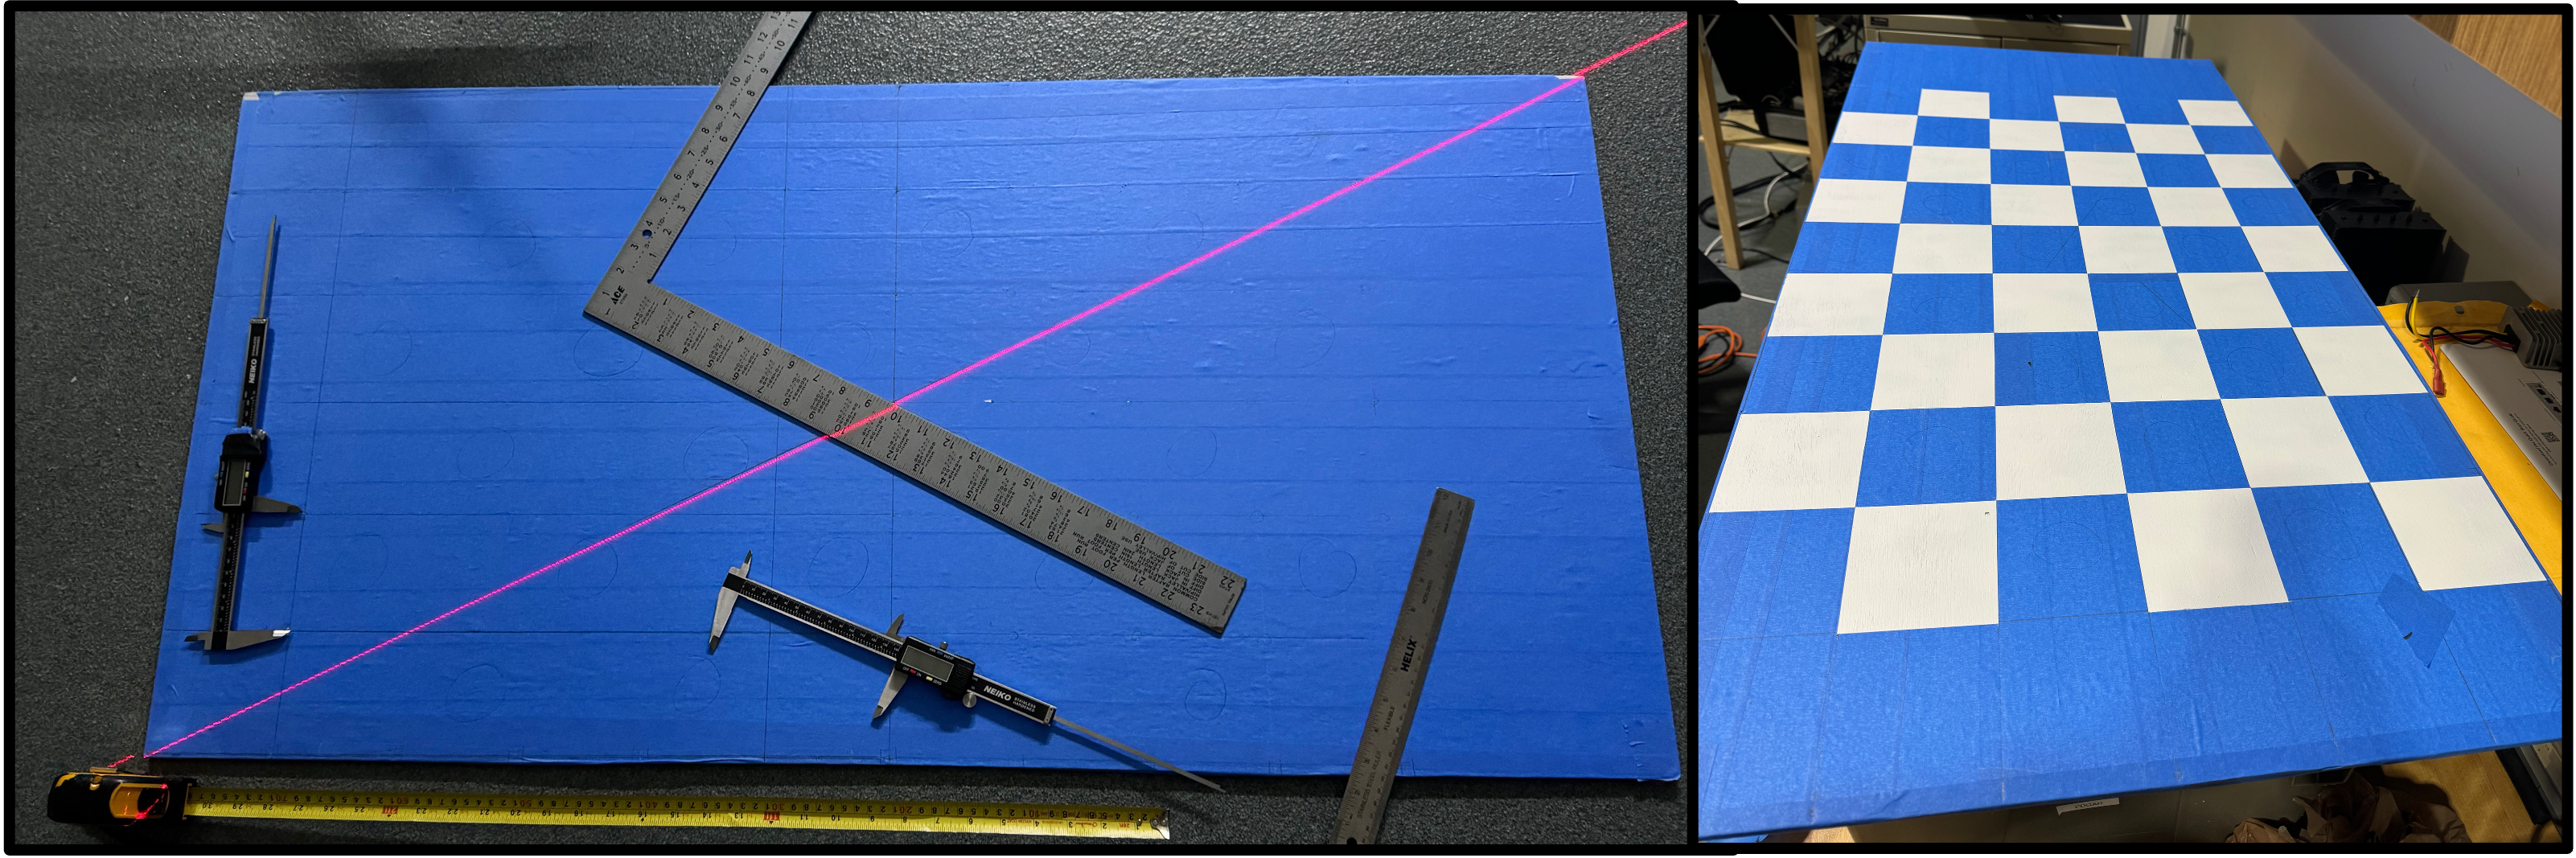
\includegraphics[width=0.9\linewidth]{Images/Checkerboard_new.png}
    \caption{New precision-painted checkerboard target used for intrinsic calibration.}
    \label{fig:checkerboard_new}
\end{figure}

\begin{figure}[htbp]
    \centering
    \includegraphics[width=0.9\linewidth]{Images/HDR_calib_error.png}
    \caption{Initial HDR camera calibration yielded a mean re-projection error of 0.63~pixels across the dataset.\textcolor{red}{reproduce graphic with larger text and landscape orientation. no need for square aspect ratio.}}
    \label{fig:HDR_calib_error}
\end{figure}

\subsubsection{Camera–LiDAR Calibration} \label{sec:camera-lidar_results}
\subfile{sections/results_camera-lidar}

\begin{figure}[htbp]
    \centering
    \includegraphics[width=0.8\linewidth]{Images/calib_checkers.png}
    \caption{Example of matched LiDAR point cloud and camera checkerboard detections used for extrinsic calibration.}
    \label{fig:calib_check}
\end{figure}

\begin{figure}[htp]
\begin{subfigure}{\textwidth}
\centering
\includegraphics[width=0.94\linewidth]{Images/LiDAR_features.png}
    \caption{}
\end{subfigure}
\bigskip
\begin{subfigure}{\textwidth}
\centering
\includegraphics[width=0.94\linewidth]{Images/LiDAR_calib_fence.png}
    \caption{}
\end{subfigure}
\caption{Vertical (red) and horizontal (green) macro-level features within the point cloud (a) are isolated (b) to support visual refinement of the camera–LiDAR alignment.}
\end{figure}

\begin{figure}[ht]
    \centering
    \includegraphics[width=0.8\linewidth]{Images/LiDAR_overlay4.png}
    \caption{Initial calibration result showing early ROI-based alignment with overlaid geometric guides for evaluation.}
    \label{fig:LiDAR_overlay4}
\end{figure}
\begin{figure}[htp]
\begin{subfigure}{\textwidth}
\centering
\includegraphics[width=0.94\linewidth]{Images/LiDAR_overlay3A.png}
    \caption{Three isolated regions of interest (ROI) in the LiDAR point cloud.}
    \label{fig:LiDAR_overlay3A}
\end{subfigure}
\bigskip
\begin{subfigure}{\textwidth}
\centering
\includegraphics[width=0.94\linewidth]{Images/LiDAR_overlay3B.png}
    \caption{}
    \label{fig:LiDAR_overlay3B.png}
\end{subfigure}
\caption{Final camera–LiDAR calibration. LiDAR ROIs containing identifiable geometry (a) are projected as red pixels onto the HDR image (b) to confirm alignment quality.}
\label{HDR_calib_final}
\end{figure}

\subsection{Temporal Calibration} \label{time_sync}
\subfile{sections/time_sync}

\subsubsection{Camera Synchronization} \label{time_sync_cam}
\subfile{sections/time_sync_cam}

\subsubsection{Network Synchronization} \label{time_sync_lan}
\subfile{sections/lan_sync}

\subsection{Results: Temporal Synchronization} \label{results_time_sync_cam}
\subfile{sections/results_time_sync}

\section{Sensor Data and Dataset} \label{sec:sensor_data_dataset}
\subfile{sections/sensor_data}



%%%%%%%%%%%%%%%%%%%%%%%%%%%%%%%%%%%%%%%%%%%%%%%%%%%
%%%%%%%%%%%%%%%%%%%%%%%%%%%%%%%%%%%%%%%%%%%%%%%%%%%
%%%%%%%%%%%%%%%%%%%%%%%%%%%%%%%%%%%%%%%%%%%%%%%%%%%
\chapter{Real-time Object Detection} \label{realtime_object_detection}
\subfile{sections/real_time_obj_det}
% a brief introduction to the chapter and overview of model selection prior to method description
% 2 to 3 paragraphs

\section{YOLO} \label{yolo}
\subfile{sections/yolo}
% This section only discusses the methods used for the YOLO object detection. 
% 3 to 4 paragraphs


\section{GB-CACHE} \label{gbcache}
\subfile{sections/gbcache}
% This section only discusses the methods used for the GB-CACHE object detection.
% 3 to 4 paragraphs


\section{Classification Results} \label{classify_results}
\subfile{sections/classify_results}

\subsection{Feature Relevance} \label{gbcache_features}
\subfile{sections/gbcache_features}

\begin{figure}
    \centering
    \includegraphics[width=0.95\linewidth]{Images/MI_analysis.png}
    \caption{Caption}
    \label{fig:MI_analysis}
\end{figure}

\begin{figure}
    \centering
    \includegraphics[width=0.95\linewidth]{Images/MI_pairwise.png}
    \caption{Caption}
    \label{fig:MI_pairwise}
\end{figure}


\section{Detection Results} \label{detect_results}
\subfile{sections/detect_results}

\section{Late Fusion} \label{late_fusion}
\subfile{sections/late_fusion}
% This section only discusses the methods used for the late fusion object detection. 

% \section{Model Performance} \label{performance}
% \subfile{sections/performance}
% This section will hold all results from analysis from the YOLO, GB cache, and late fusion techniques. 

\subsection{YOLO} \label{performance_yolo}
\subfile{sections/performance_yolo}

\subsection{GB-CACHE} \label{performance_gbcache}
\subfile{sections/performance_gbcache}






\chapter{Conclusions}
% This chapter will synthesize findings from all three research objectives:
% - Summary of comparative performance results between LiDAR and vision systems
% - Calibration and synchronization framework effectiveness
% - Real-time processing capability validation
% - Implications for ASV perception system design
% - Contribution to maritime autonomous systems knowledge

% \section{Research Objective Achievement Summary}
% \subfile{}
% Placeholder for objective completion summary

% \section{Performance Comparison Findings}
% \subfile{}
% Placeholder for key comparative analysis conclusions

% \section{Implications for ASV System Design}
% \subfile{}
% Placeholder for practical design guidance conclusions


\chapter{Recommendations and Future Work} \label{chap:recommendations}
% \subfile{sections/real_time_obj_det}
% a brief introduction to the chapter 

% \section{Recommendations} \label{sec:recommendations}
% \subfile{)

\section{Future Work} \label{futurework}

% This dual-system configuration facilitated the transition of Minion's software during the period of this research.
% \ac{ROS} 1 was the operational framework for all research and data collected in this study, however, \ac{ROS} 1 has entered end-of-life for active development.
% Consequently, Minion’s software architecture was gradually migrated to \ac{ROS} 2, which introduces substantial improvements in real-time performance, memory management, and inter-process communication.
% In contrast to ROS 1’s reliance on a centralized message broker, ROS 2 employs a Data Distribution Service-based communication layer that reduces latency and memory overhead through zero-copy data handling and improved resource allocation.
% Maintaining one system on ROS 1 while transitioning the other to ROS 2 allowed incremental software migration without interrupting field operations—laying the groundwork for future runtime performance improvements anticipated in Section~\ref{futurework}.


% \section{ASV Perception System Design Recommendations}
% \subfile{}
% Placeholder for design guidance recommendations

% \section{Future Research Directions}
% \subfile{}
% Placeholder for future work recommendations

% \section{Technology Transfer Opportunities}
% \subfile{}
% Placeholder for practical application recommendations




% \printbibliography
% \bibliographystyle{plainnat} - Most recent
\bibliographystyle{IEEEtranN} % natbib-compatible numeric IEEE style
% \bibliography{References}
\bibliography{Dissertation,extra_cite}

\backmatter


\chapter{Image Transform} \label{img_tform}
\subfile{sections/img_tform}

\chapter{Video Encoding and Timestamp Pipeline} \label{append_video_pipeline}

\begin{figure}[htbp]
\centering
\includegraphics[width=0.95\textwidth]{Images/gstreamer_block.png}
\caption{Block diagram of the NVIDIA Jetson's video pipeline. Green rectangles represent video data entering or leaving the pipeline, while red rectangles indicate local file creation. Light-blue rectangles with chamfered corners denote timestamp acquisition and application operations within the pipeline.}
\label{fig_video_pipeline}
\end{figure}


% \chapter{test 2}

% \begin{figure}[htbp]
%        \centering
%        % TikZ Flowchart for GStreamer HDR Pipeline
% Drop-in code for Overleaf
% Requires: \usepackage{tikz}
%          \usetikzlibrary{shapes.geometric, arrows}

\tikzstyle{process} = [rectangle, minimum width=3cm, minimum height=1cm, text centered, draw=black, fill=white, text width=3cm]
\tikzstyle{timestamp} = [rectangle, minimum width=3cm, minimum height=1cm, text centered, draw=red, line width=1.5pt, fill=white, text width=3cm]
\tikzstyle{queue} = [rectangle, minimum width=2.5cm, minimum height=0.8cm, text centered, draw=blue, line width=1.2pt, fill=white, text width=2.5cm]
\tikzstyle{output} = [rectangle, minimum width=2.5cm, minimum height=1cm, text centered, draw=green!60!black, line width=1.2pt, fill=white, text width=2.5cm, rounded corners]
\tikzstyle{decision} = [diamond, minimum width=2cm, minimum height=1cm, text centered, draw=black, fill=white, aspect=2]
\tikzstyle{arrow} = [thick,->,>=stealth]

\begin{tikzpicture}[node distance=2cm]

% Source
\node (source) [process] {\textbf{v4l2src / videotestsrc} \\ YUY2, 2880x1860@60fps \\ do-timestamp=TRUE};

% Timestamp Probe 1
\node (ts1) [timestamp, below of=source] {\textbf{TIMESTAMP PROBE \#1} \\ timestamp\_probe\_cb \\ Adds CustomTimestampMeta \\ gettimeofday() $\rightarrow$ ms};

% Tee
\node (tee) [decision, below of=ts1, yshift=-0.5cm] {\textbf{TEE (Splits 3x)}};

% Stream Branch (left)
\node (qs) [queue, below of=tee, xshift=-8cm, yshift=-1.5cm] {\textbf{queue\_stream} \\ {[BUFFER QUEUE]}};
\node (vr) [process, below of=qs] {\textbf{videorate} \\ 60fps $\rightarrow$ 5fps};
\node (nvc1) [process, below of=vr] {\textbf{nvvidconv} \\ YUY2 $\rightarrow$ I420 \\ NVMM memory};
\node (h264e) [process, below of=nvc1] {\textbf{nvv4l2h264enc} \\ H264 encode \\ bitrate=calc \\ insert-sps-pps=true};
\node (sei) [timestamp, below of=h264e] {\textbf{TIMESTAMP PROBE \#2} \\ sei\_insert\_probe\_cb \\ Reads CustomTimestampMeta \\ Inserts SEI NAL unit};
\node (h264p) [process, below of=sei] {\textbf{h264parse} \\ Parse H264 stream};
\node (rtp) [process, below of=h264p] {\textbf{rtph264pay} \\ RTP payload \\ config-interval=1 \\ mtu=1400};
\node (udp) [output, below of=rtp] {\textbf{udpsink} \\ host=201.7.90.18 \\ port=5603 \\ sync=false};

% Record Branch (middle)
\node (qr) [queue, below of=tee, yshift=-1.5cm] {\textbf{queue\_record} \\ {[BUFFER QUEUE]}};
\node (nvc2) [process, below of=qr] {\textbf{nvvidconv} \\ YUY2 $\rightarrow$ I420 \\ NVMM memory};
\node (h265e) [process, below of=nvc2] {\textbf{nvv4l2h265enc} \\ H265 encode \\ bitrate=80Mbps \\ iframeinterval=1};
\node (h265p) [process, below of=h265e] {\textbf{h265parse} \\ Parse H265 \\ byte-stream};
\node (split) [output, below of=h265p, yshift=-1cm] {\textbf{splitmuxsink} \\ muxer=qtmux \\ Split @120s \\ /mnt/logs/hdr-0/ \\ hdr-0-\{time\}-\{n\}.mp4};

% CSV Branch (right)
\node (qc) [queue, below of=tee, xshift=8cm, yshift=-1.5cm] {\textbf{queue} \\ {[BUFFER QUEUE]}};
\node (id) [process, below of=qc] {\textbf{identity} \\ csv\_identity \\ signal-handoffs=true};
\node (csv) [timestamp, below of=id] {\textbf{TIMESTAMP LOGGER} \\ csv\_handoff\_handler \\ Reads CustomTimestampMeta \\ Logs: frame\#,timestamp};
\node (csvf) [output, below of=csv, xshift=-2.5cm, yshift=-0.5cm] {\textbf{CSV Files} \\ /mnt/logs/hdr-0/ \\ hdr-0-\{time\}-\{n\}.csv \\ Split @120s};
\node (fake) [output, below of=csv, xshift=2.5cm, yshift=-0.5cm] {\textbf{fakesink} \\ discard};

% Arrows
\draw [arrow] (source) -- (ts1);
\draw [arrow] (ts1) -- node[anchor=east, xshift=-0.3cm] {[BUFFER + Metadata]} (tee);

% Stream branch arrows
\draw [arrow] (tee) -| node[anchor=south, yshift=0.3cm, xshift=-4cm] {Stream Branch} (qs);
\draw [arrow] (qs) -- (vr);
\draw [arrow] (vr) -- (nvc1);
\draw [arrow] (nvc1) -- (h264e);
\draw [arrow] (h264e) -- (sei);
\draw [arrow] (sei) -- node[anchor=east, xshift=-0.3cm] {[H264 + SEI NAL]} (h264p);
\draw [arrow] (h264p) -- (rtp);
\draw [arrow] (rtp) -- node[anchor=east, xshift=-0.3cm] {[RTP Packets]} (udp);

% Record branch arrows
\draw [arrow] (tee) -- node[anchor=east, xshift=-0.3cm] {Record Branch} (qr);
\draw [arrow] (qr) -- (nvc2);
\draw [arrow] (nvc2) -- (h265e);
\draw [arrow] (h265e) -- (h265p);
\draw [arrow] (h265p) -- (split);

% CSV branch arrows
\draw [arrow] (tee) -| node[anchor=south, yshift=0.3cm, xshift=4cm] {CSV Branch} (qc);
\draw [arrow] (qc) -- (id);
\draw [arrow] (id) -- (csv);
\draw [arrow] (csv) -- (csvf);
\draw [arrow] (csv) -- (fake);

\end{tikzpicture}

%        \caption{GStreamer pipeline architecture for HDR camera streaming, 
%                 recording, and timestamp logging.}
%        \label{fig:hdr_pipeline}
%    \end{figure}


\end{document}